\documentclass[aip,amsmath,amssymb,reprint, jcp]{revtex4-1}
\usepackage{tikz}
\usepackage{graphicx}% Include figure files
\usepackage{dcolumn}% Align table columns on decimal point
\usepackage{bm}% bold math
%My packages start
%\usepackage{subfig}
\usepackage{multirow}					
\usepackage{array}
%\usepackage{booktabs}
\usepackage{footnote} 
\usepackage{subcaption}
\newcommand{\angstrom}{\text{\normalfont\AA}}
\usepackage{booktabs}
\usepackage{float}
\usepackage{mathtools}
\usepackage{color}
\usepackage{natmove}
\newcommand{\comment}[1]{\noindent \textcolor{blue}{#1}}

% Extra packages (MP):

\usepackage{tikz}
\usetikzlibrary{shapes,arrows,decorations.markings}

\newcommand*{\citen}[1]{%
  \begingroup
    \romannumeral-`\x % remove space at the beginning of \setcitestyle
    \setcitestyle{numbers}%
    \cite{#1}%
  \endgroup   
}


%My packages end
%\usepackage[mathlines]{lineno}% Enable numbering of text and display math
%\linenumbers\relax % Commence numbering lines

\begin{document}

\title[]{Stability and Reactivity of Pt-Oxide Nano Clusters}
\author{Siva Chiriki}
\author{}
\author{B.\ Hammer}
\email{hammer@phys.au.dk}
\affiliation{ 
Department of Physics and Astronomy, Aarhus University, DK-8000 Aarhus C, Denmark.
}
% \homepage{phys.au.dk}
 
\date{\today}% It is always \today, today,
             %  but any date may be explicitly specified

\begin{abstract}

\end{abstract}
\maketitle

% Introduction
\section{\label{sec:introduction}Introduction}

\section{Pt$_7$ Isomers}


\begin{figure}
 \begin{subfigure}
 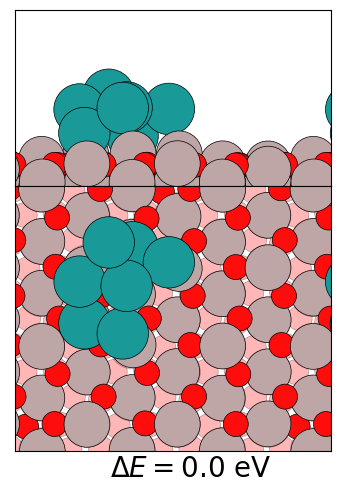
\includegraphics[width=0.90\textwidth]{Pt7_Al2O3_Lowlying_DFTrelxed_0.png}}
 \end{subfigure}
 \begin{subfigure}
 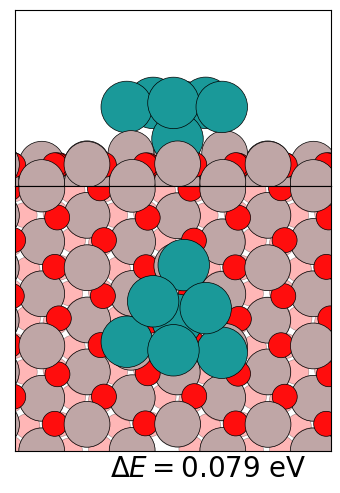
\includegraphics[width=0.90\textwidth]{Pt7_Al2O3_Lowlying_DFTrelxed_1.png}}
 \end{subfigure}
 \begin{subfigure}
 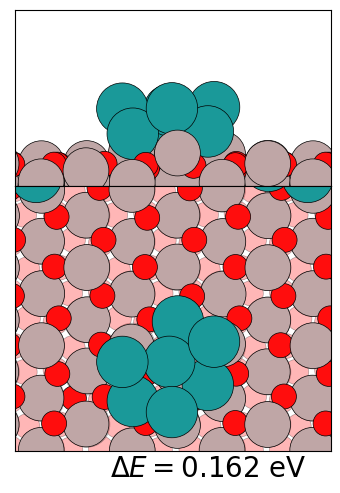
\includegraphics[width=0.90\textwidth]{Pt7_Al2O3_Lowlying_DFTrelxed_2.png}}
 \end{subfigure}
 \begin{subfigure}
 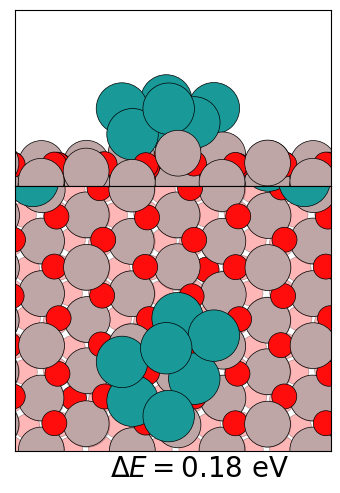
\includegraphics[width=0.90\textwidth]{Pt7_Al2O3_Lowlying_DFTrelxed_3.png}}
 \end{subfigure}
 \begin{subfigure}
 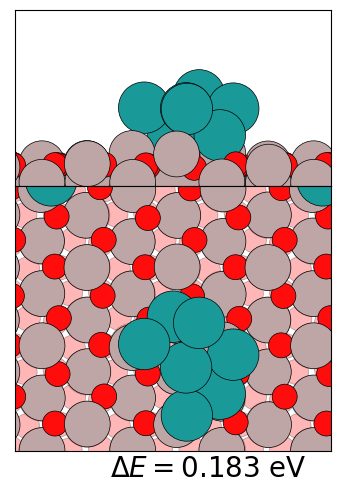
\includegraphics[width=0.90\textwidth]{Pt7_Al2O3_Lowlying_DFTrelxed_4.png}}
 \end{subfigure}
\label{fig:iterativeconvergenceSiO2}
\end{figure}   


%\section{Acknowledgements}
We acknowledge support from VILLUM Fonden (Investigator grant, project no. 16562).

%\section{References}
%\nocite{*}
%\bibliography{bib}

\end{document}


